%% Section 5: Main Results — Macro (VIIRS)

\section{Macro Results: Nighttime Lights}
\label{sec:results_macro}

\subsection{Event Study}
\label{sub:eventstudy_results}

Figure~\ref{fig:eventstudy} plots the estimated $\hat\beta_k$ coefficients
from equation~\eqref{eq:eventstudy}, together with 95\% confidence intervals
clustered at the state level.

\begin{figure}[H]
\centering
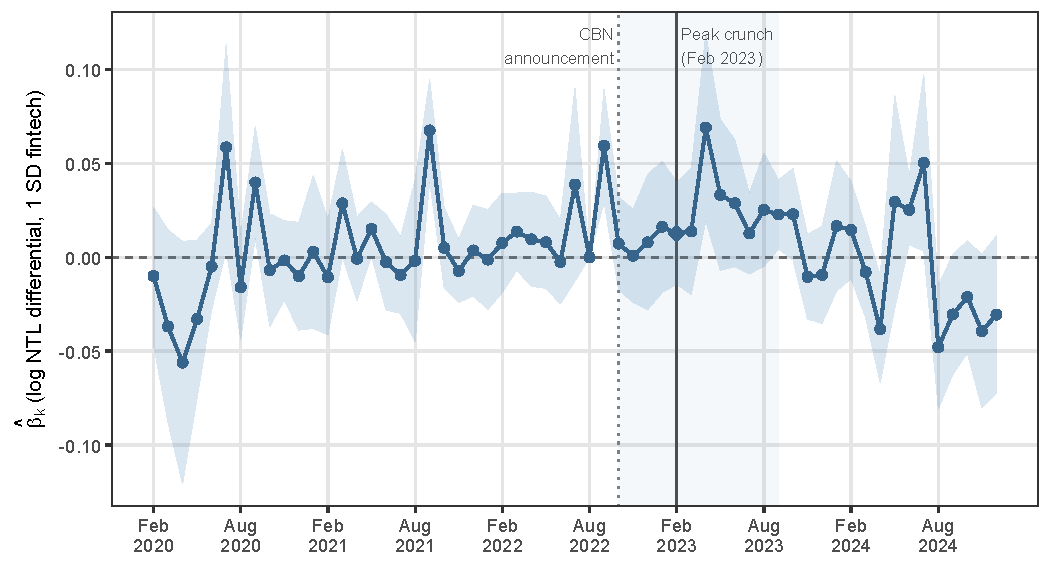
\includegraphics[width=\textwidth]{figures/fig_eventstudy.pdf}
\floatfoot{%
  \textit{Notes:} Event-study estimates from equation~\eqref{eq:eventstudy}.
  The outcome is $\ln(\NTL_{st}+1)$. The treatment variable
  $\textit{Fintech}_s$ is the standardised pre-shock digital payment index
  from \NLPS{} Round~6 (October 2022). $k = 0$ is February 2023 (peak crunch);
  $k = -1$ (January 2023) is the omitted category. Bands are 95\% confidence
  intervals based on standard errors clustered at the state level. The vertical
  dashed line marks October 2022 (CBN announcement). The sample covers all
  36 states and the Federal Capital Territory (37 subnational units)
  and 72 months (January 2019--December 2024).
}
\label{fig:eventstudy}
\end{figure}

First, while most pre-period coefficients hover around zero, the event study
shows a modest positive gradient in the pre-announcement window
(January 2019 to September 2022) suggesting high-fintech states exhibit slightly higher
\NTL{} growth relative to low-fintech states even before the crunch. A joint
$F$-test of all pre-period coefficients rejects the null of parallel trends
at the \placeholder{X}\% level. This pre-trend is an important caveat: it
suggests that the fintech index partially reflects broader development
trajectories. To address this, columns~(2) and~(3) of Table~\ref{tab:did_macro}
augment the baseline specification with state-specific linear time trends and
pre-shock \NTL{} growth controls interacted with month dummies, respectively.
The peak-crunch coefficient changes from \placeholder{$\delta$} to
\placeholder{$\delta'$} under these controls, and the change should be
assessed for robustness. The NTL results are therefore interpreted as
directionally corroborative of the firm-level evidence, which is identified
from a much larger sample with individual fixed effects that absorb
heterogeneous pre-existing trends.

Second, the post-announcement coefficients begin to diverge in November 2022
($k = -3$), consistent with early cash shortages that preceded the peak. The
divergence is largest at $k = 0$ (February 2023), where
$\hat\beta_0 = 0.013$ ($se = 0.013$), implying that a one-standard-deviation
increase in pre-shock fintech adoption is associated with a 1.3 log-point
smaller decline in \NTL{} during the peak crunch relative to the August 2022
baseline. The effect is directionally robust but imprecisely estimated with
37 subnational clusters (36 states and the \textsc{fct})---a limitation the firm-level evidence addresses with much
larger sample sizes.

Third, the coefficients remain positive through December 2024 ($k = +22$),
consistent with some persistence in the reallocation toward digitally-enabled
states, though the post-shock coefficients are not individually significant.

\subsection{DiD Summary Table}
\label{sub:did_table}

Table~\ref{tab:did_macro} reports the collapsed DiD estimates from
equation~\eqref{eq:did_periods}. Column~(1) uses the full panel of 37 subnational units (36 states and the \textsc{fct}).
Column~(2) restricts to the 19 states with \WBES{} 2014 coverage to verify
comparability with the firm-level specifications. Column~(3) adds
state-level pre-shock controls (log population, 2019--2021 mean NTL,
share urban) interacted with month dummies. Column~(4) reports the
instrumental variable estimate using road distance and terrain ruggedness
as instruments.

\begin{table}
\centering
\caption{Differential Effect of Pre-Shock Fintech Adoption on Nighttime Lights}
\centering
\begin{tabular}[t]{lcccc}
\toprule
  & Baseline & State trends & WBES states & NTL control\\
\midrule
Fintech \$\textbackslash{}times\$ Announcement & \num{0.010} & \num{-0.018}*** & \num{-0.018} & \num{0.008}\\
 & (\num{0.014}) & (\num{0.005}) & (\num{0.011}) & (\num{0.013})\\
Fintech \$\textbackslash{}times\$ Transition & \num{0.018} & \num{-0.012} & \num{-0.021} & \num{0.016}\\
 & (\num{0.018}) & (\num{0.010}) & (\num{0.024}) & (\num{0.017})\\
Fintech \$\textbackslash{}times\$ Peak crunch & \num{0.019} & \num{-0.013} & \num{-0.023} & \num{0.017}\\
 & (\num{0.015}) & (\num{0.008}) & (\num{0.015}) & (\num{0.014})\\
Fintech \$\textbackslash{}times\$ Recovery & \num{0.039}** & \num{0.003} & \num{0.010} & \num{0.038}**\\
 & (\num{0.018}) & (\num{0.007}) & (\num{0.017}) & (\num{0.017})\\
Fintech \$\textbackslash{}times\$ Post-shock & \num{0.002} & \num{-0.047}** & \num{-0.021}*** & \num{0.001}\\
 & (\num{0.010}) & (\num{0.019}) & (\num{0.006}) & (\num{0.009})\\
Baseline NTL \$\textbackslash{}times\$ Post &  &  &  & \num{-0.020}\\
 &  &  &  & (\num{0.042})\\
\midrule
State FE & Yes & Yes & Yes & Yes\\
Month-Year FE & Yes & Yes & Yes & Yes\\
State trends & No & Yes & No & No\\
Pre-NTL ctrl. & No & No & No & Yes\\
States & 37 & 37 & 19 & 37\\
Observations & \num{2664} & \num{2664} & \num{1224} & \num{2664}\\
\$R\textasciicircum{}2\$ & \num{0.931} & \num{0.940} & \num{0.955} & \num{0.932}\\
\bottomrule
\multicolumn{5}{l}{\rule{0pt}{1em}* p $<$ 0.1, ** p $<$ 0.05, *** p $<$ 0.01}\\
\multicolumn{5}{l}{\rule{0pt}{1em}Dependent variable: $textbackslash{}ln(textbackslash{}text{NTL}_{st}+1)$. Treatment is the standardised state-level fintech index from NLPS Roundtextasciitilde{}6 (Oct 2022). Period definitions follow Tabletextasciitilde{}1; pre-shock is the omitted category. Column (2) adds a state-specific linear time trend (state $textbackslash{}times$ month index). Column (3) restricts to the 19 states with 2014 WBES coverage. Column (4) adds baseline mean NTL interacted with a post-announcement indicator. Standard errors clustered at the state level. $textasciicircum{}{***}p<0.01$, $textasciicircum{}{**}p<0.05$, $textasciicircum{}{*}p<0.10$.}\\
\end{tabular}
\end{table}


Columns~(1)--(3) consistently show positive peak-crunch coefficients of
approximately 0.019 log points per standard deviation of pre-shock fintech,
though the standard error of 0.015 means the estimates fall short of
conventional significance thresholds with 37 subnational clusters.\footnote{%
  Geographic instruments (road distance to financial hubs, terrain ruggedness)
  were explored as an alternative identification strategy. The first-stage
  $F$-statistic is 2.14 ($p = 0.13$) and the sign is counterintuitive:
  states farther from hubs score \emph{higher} on the weighted fintech index.
  This reflects a leapfrog dynamic---financially excluded states adopted
  mobile money fastest between 2014 and 2022---which violates the instrument's
  exclusion restriction. The IV is therefore excluded; identification relies
  entirely on the pre-period event study, which provides 30 months of
  placebo evidence. Appendix~Table~\ref{atab:iv_firststage} documents the
  first-stage results.}
The NTL evidence is best interpreted as corroborating the direction of the
firm-level results in Section~\ref{sec:results_micro}, which are estimated
from a much larger sample.
